\documentclass[11pt]{article}

\usepackage[margin=1.05in]{geometry}
\usepackage{graphicx}
\usepackage{booktabs}
\usepackage{amsmath}
\usepackage{amssymb}
\usepackage{enumitem}
\usepackage{parskip}
\usepackage{xcolor}
\usepackage[colorlinks=true,
            linkcolor=blue!40!black,
            urlcolor=blue!40!black,
            pdftitle={Possibilistic Decomposition of a Tomographic Inversion},
            pdfauthor={Aaron Green}]{hyperref}

\setlist{itemsep=3pt,topsep=5pt,parsep=0pt}
\emergencystretch=3em   % absorb the odd overfull line (long \texttt tokens)
\newcommand{\amin}{a_{\min}}
\newcommand{\amax}{a_{\max}}
\newcommand{\file}[1]{\texttt{#1}}

\title{\textbf{Possibilistic Decomposition of a Tomographic Inversion}\\[6pt]
  {\large\itshape Separating data-forced structure from regularization
  artifact}}
\author{Aaron Green}
\date{Draft prepared for Zagid Abatchev \;---\; 2026-05-17}

\begin{document}
\maketitle

\section*{What this is}

A tomographic image is not a picture of the Earth. It is the output of a long
chain of lossy, selective steps---sparse rays, a simplified forward model, a
parameterization, a regularizer, an optimizer---and what survives that chain is
not the structure but a \emph{filtered residue} of it. You and I have said as
much to each other already. The practical question that framing forces is the
one this note is about:

\begin{quote}
\itshape\bfseries Given a finished inversion, which features did the data
force, and which did the regularization invent?
\end{quote}

Standard practice does not answer that question. It picks a damping value,
returns one model, and attaches a posterior covariance---and every part of that
is conditional on the damping choice. Your own thesis says it plainly:
``there is no simple solution for regularization, and optimization of damping
conditions remains a highly parametrization and input dependent problem''
(ZTM/TFM, \S11).

This note proposes a different reading of an inversion---a
\textbf{possibilistic} one---and demonstrates it end-to-end on synthetic
travel-time tomography with two forward operators, straight-ray and Eikonal. It
is a methods communication and a draft; the demonstrations are synthetic;
nothing here is claimed as proven. What I am claiming is that the reading is
sound, that it is implemented and validated against known ground truth, and
that the place it stops working cleanly is a real open problem worth our
working on together.

\section{The problem: a damping choice is not a fact}

Tomographic inversion is ill-posed. Many models fit the data within noise. To
return \emph{one} model you must regularize---damp, smooth, prefer a
reference---and the model you get is as much a property of that choice as of
the data.

The honest consequence: a feature in a tomographic image belongs to one of
three classes, and they are not the same kind of thing.

\begin{table}[htbp]
\centering
\renewcommand{\arraystretch}{1.25}
\begin{tabular}{@{}l p{0.72\linewidth}@{}}
\toprule
\textbf{Class} & \textbf{Meaning} \\
\midrule
\textbf{Forced} & Present in \emph{every} model consistent with the data and
the hard physical bounds. Data-determined. Independent of the damping choice. \\
\textbf{Forbidden} & Present in \emph{no} such model. \\
\textbf{Measure-dependent} & Present in \emph{some} consistent models and
absent in others. The data do not determine it---which sign or structure you
see is set by the regularization. Such a feature may still be physically real:
measure-dependence diagnoses \emph{underdetermination}, not falsehood. \\
\bottomrule
\end{tabular}
\end{table}

A posterior covariance does not draw this line. It reports a spread \emph{under
one prior and one damping}; it cannot tell you that a given feature would
vanish under a different, equally defensible choice. The damping problem of
\S11 is, in this language, a symptom of reading an inversion through the wrong
layer: it is the search for the ``right'' measure-layer choice to extract a
model, when the features that \emph{depend} on that choice are exactly the ones
the data does not determine.

\section{The possibilistic frame}

The distinction in \S1 is the \textbf{possibilistic / probabilistic} split,
taken from the two-layer discipline of the Closure Forces Structure programme
(\file{inverse\_born\_methodology.md}) and carried over to inversion:

\begin{itemize}
\item The \textbf{possibilistic layer} asks what is \emph{forced or forbidden}
  by the data and the hard physical constraints alone. Its answers are
  unconditional---they do not depend on a prior, a damping value, or a measure.
\item The \textbf{probabilistic layer} asks how a measure distributes weight
  over what the possibilistic layer permits. Its answers are conditional on
  that measure.
\end{itemize}

A posterior covariance is a probabilistic-layer object. The possibilistic
layer is the one that answers the \S1 question, and it is the one standard
tomography leaves on the table.

One clarification carries the rest. Throughout, $F$ is the \emph{hard}
admissibility set---every model that fits within the noise tolerance and obeys
the hard physical bounds---and the probabilistic layer is taken as conditional
on that admissibility. With a smooth likelihood a posterior need not vanish
sharply outside $F$; the two-layer reading treats $F$ as the tolerance-defined
region and a measure $\mu$ as a measure on it. Every ``measure on $F$'' below---and
every bound stated in terms of ``$F$'s extent,'' including
Figure~\ref{fig:compose}'s---is a claim about admissible $\mu$ in that
conditional sense, not about an untruncated smooth-likelihood posterior.

The split has a natural geometry, and the next three figures build it up one
idea at a time.

\textbf{Figure~\ref{fig:feasible} --- the feasible set.} The data and the hard
constraints do not pick out a model; they pick out a \emph{set} $F$ of
models---every model that fits within noise and respects the bounds. $F$ is a
set, not a probability density---the figures shade it only to mark the region.
Project $F$ onto a feature's axis and the feature falls into one of two classes. It is
\textbf{forced} when the projection lies entirely on one side of zero: every
model consistent with the data agrees on its sign, and no prior is needed to
settle it. It is \textbf{measure-dependent} when the projection straddles zero:
the data leave the sign open, and any single value reported there is fixed by
the measure you add, not by the data.

\begin{figure}[htbp]
\centering
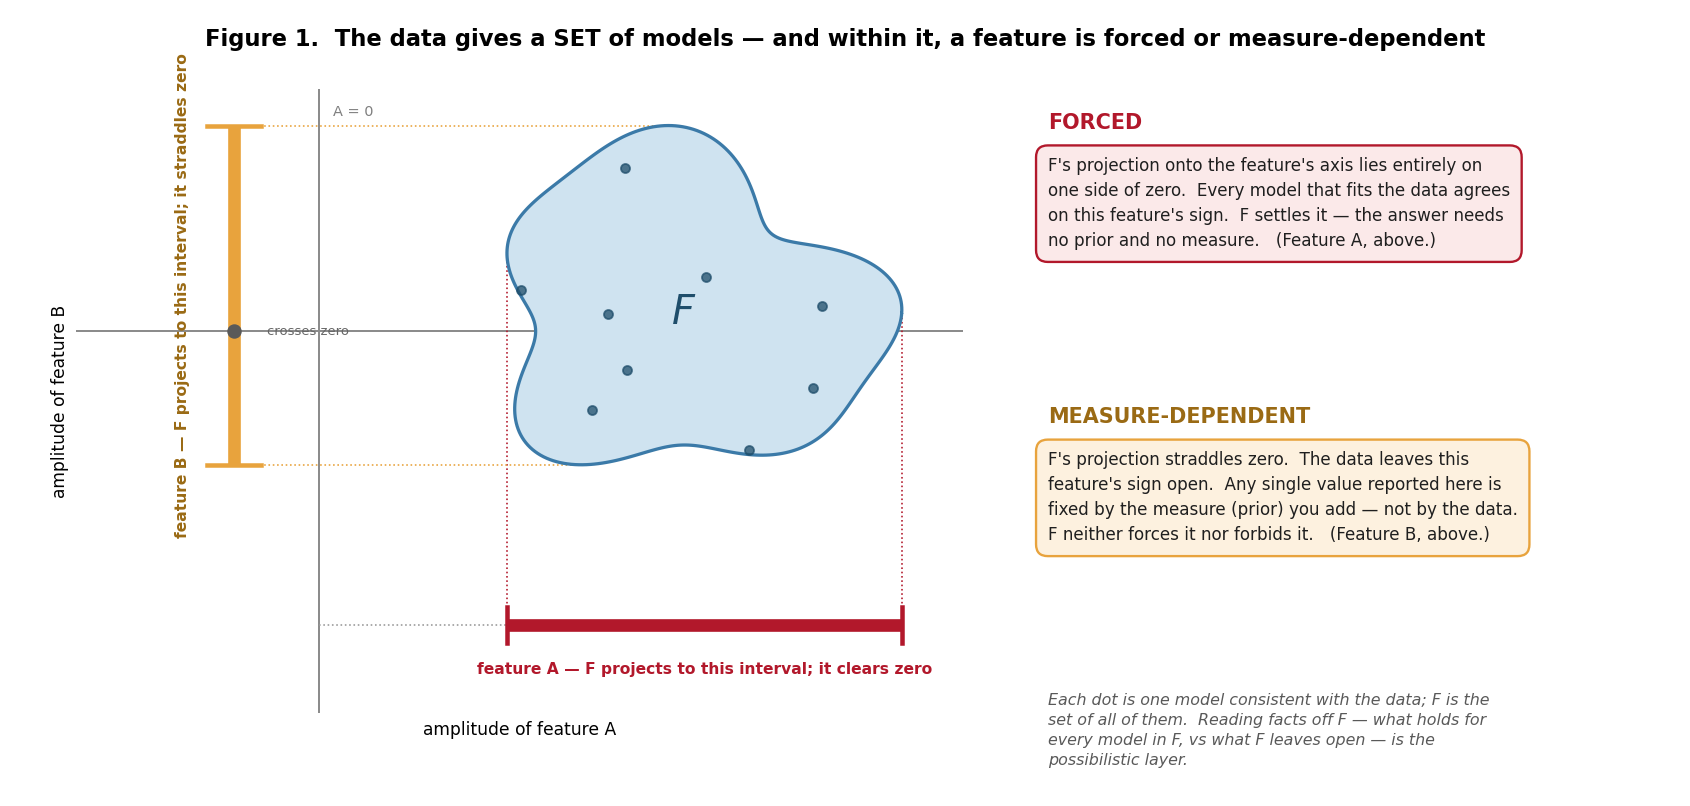
\includegraphics[width=\linewidth]{fig_feasible_set.png}
\caption{The data give a set, not a point. A feature is forced when $F$'s
projection clears zero and measure-dependent when it straddles zero---the two
terms this note turns on, defined geometrically.}
\label{fig:feasible}
\end{figure}

\textbf{On the word ``possibilistic.''} I use it in a deliberately narrow
sense---the crisp-set limit of possibility theory, equivalently a set-valued
feasibility reading, not a graded possibility distribution. $F$ is an ordinary
feasible set: a model is in it or
it is not. A feature is \emph{forced} exactly when a fact holds for every model
in $F$ (necessity~1, in possibility-theory terms) and \emph{measure-dependent}
when $F$ neither forces nor forbids it. No fuzzy membership is invoked; the only
structure used is the set $F$ and the all-or-nothing quantifier over it.

\textbf{Figure~\ref{fig:reports} --- two reports.} The same $F$ can be turned
into a reported answer two ways. The \emph{possibilistic report} uses exactly
$F$: forced features pinned to a sign, measure-dependent features returned as
intervals---no more information than $F$ carries, and no less. The
\emph{Bayesian report} uses $F$ plus a measure $\mu$---it places $\mu$ on $F$
and reports its mean and credible interval. $\mu$ is information beyond $F$, and
two defensible choices of $\mu$ can disagree on a measure-dependent feature's
sign, so that choice needs a justification of its own. On a forced feature the
two reports agree; the divergence is confined to the measure-dependent ones.

\begin{figure}[htbp]
\centering
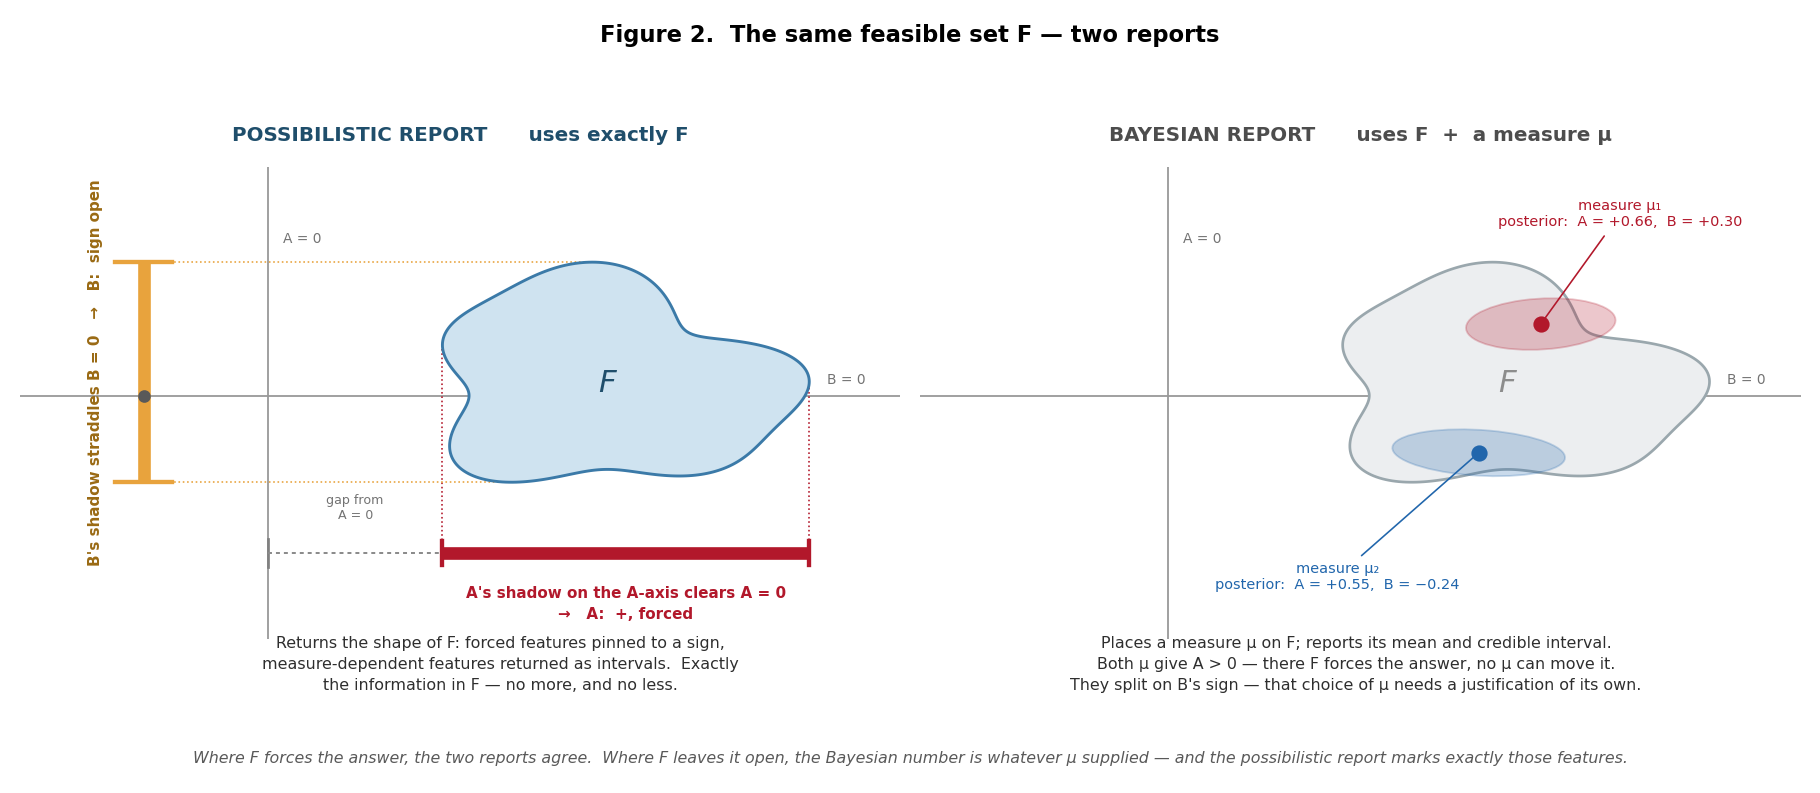
\includegraphics[width=\linewidth]{fig_two_reports.png}
\caption{Two reports from one feasible set. Possibilistic: use exactly $F$.
Bayesian: use $F$ plus a measure $\mu$---defensible $\mu$ agree where $F$ forces
the answer and can conflict where it does not.}
\label{fig:reports}
\end{figure}

\textbf{Figure~\ref{fig:compose} --- the layers compose.} The two are not
rivals run side by side; they compose in sequence. The possibilistic layer runs
first and bounds which measures are admissible---a measure is admissible only if
it is supported on $F$. The Bayesian layer then runs inside that bound: across
all admissible measures, the \emph{attainable range of reported answers}---the
measure-uncertainty---cannot exceed $F$'s extent. On a forced feature
that bound clears zero, so no admissible measure can move the sign; on a
measure-dependent feature it straddles zero and the sign is genuinely open.
Possibilism does not compete with Bayes---it brackets it.

\begin{figure}[htbp]
\centering
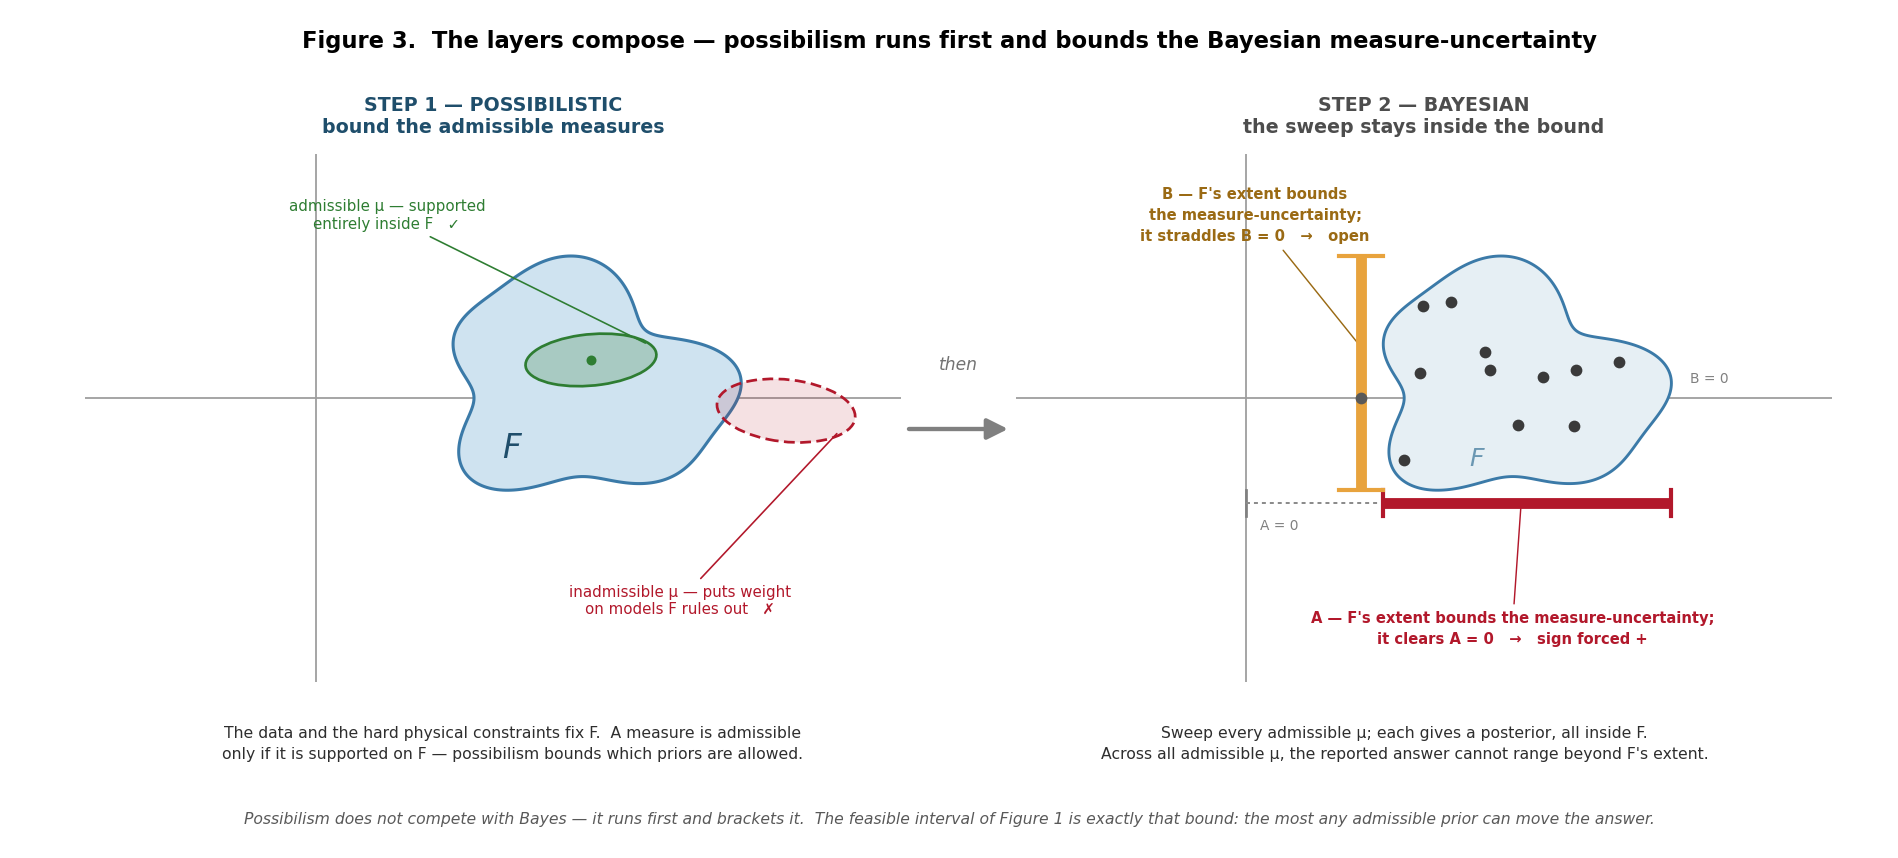
\includegraphics[width=\linewidth]{fig_bounded_uncertainty.png}
\caption{The layers compose. Possibilism runs first and bounds the admissible
measures; the Bayesian sweep then stays inside that bound. The feasible interval
below is exactly that bound.}
\label{fig:compose}
\end{figure}

The object that carries the possibilistic content is the \textbf{feasible
interval}. Take an ensemble of models that each fit the data within noise and
respect the hard bounds. For each cell, record the interval $[\amin,\amax]$ of
the anomaly across the ensemble. That interval is $F$ projected onto the cell's
axis---exactly the bound Figure~\ref{fig:compose} draws:

\begin{itemize}
\item $\amin > 0$ everywhere in the ensemble $\rightarrow$
  \textbf{forced-high} (no data-consistent model makes this cell
  non-positive);
\item $\amax < 0$ $\rightarrow$ \textbf{forced-low};
\item the interval straddles zero $\rightarrow$ \textbf{measure-dependent}
  (the sign itself is not data-forced);
\item the interval sits inside a small band around zero $\rightarrow$
  \textbf{forced-quiet}.
\end{itemize}

Figure~\ref{fig:schematic} puts the classification on a concrete ensemble. The
same ensemble, read two ways: the probabilistic reading collapses it to a mean
and an error band; the possibilistic reading keeps the feasible interval and
classifies it. The big feature is forced; the flanks and the small bump are
measure-dependent---and the probabilistic band does not distinguish them.

\begin{figure}[htbp]
\centering
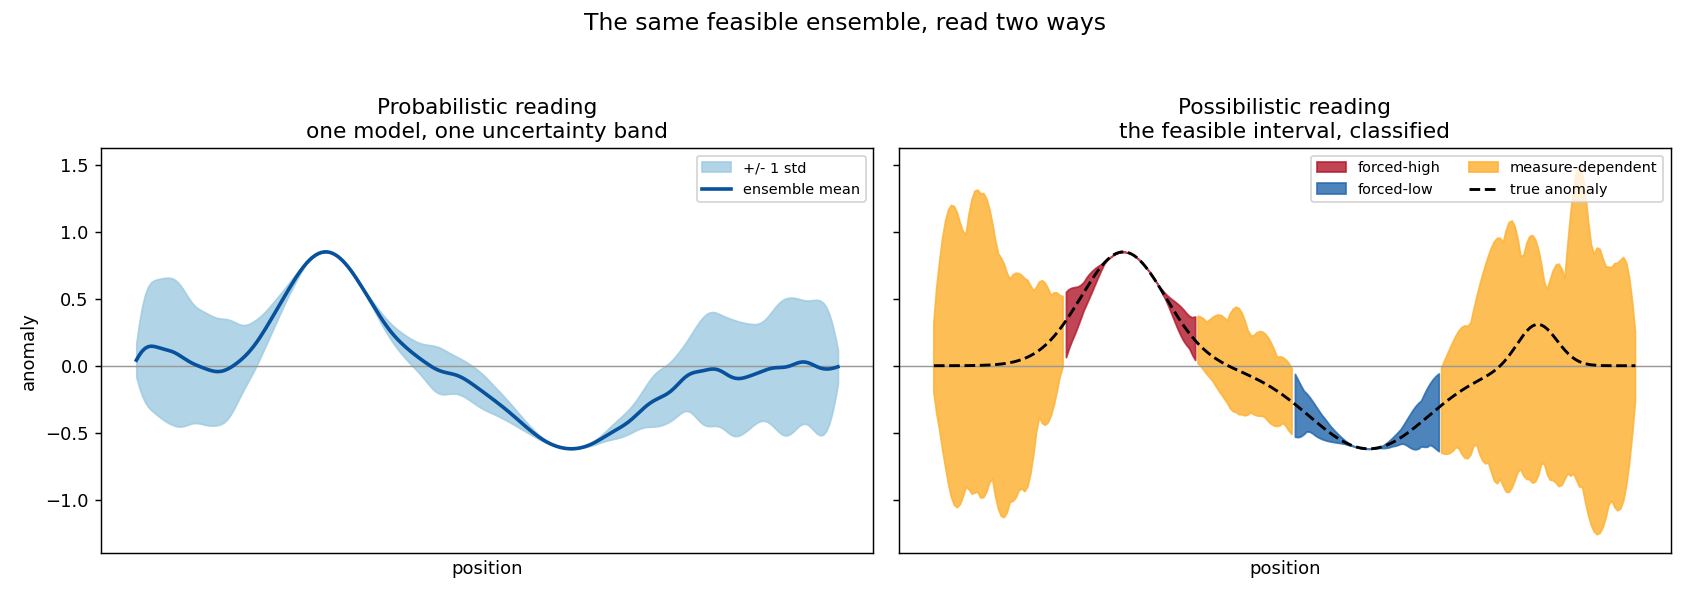
\includegraphics[width=\linewidth]{fig_schematic.png}
\caption{The same feasible ensemble, read two ways. Left: one model, one
uncertainty band. Right: the feasible interval, classified into
forced-high / forced-low / measure-dependent.}
\label{fig:schematic}
\end{figure}

\paragraph{On prior art --- said straight.}
This is not unprecedented, and pretending otherwise would not survive five
minutes of your scrutiny. Computing bounds on what a model \emph{can} be,
rather than a single estimate, is the spirit of Backus--Gilbert extremal
inversion (1968); the under-determined directions are the null space of
resolution analysis; multi-model joint coupling has the Gramian-constraint
literature (Zhdanov, 2012 onward). And a transdimensional / reversible-jump
MCMC posterior ensemble (Bodin \& Sambridge, 2009) already \emph{contains} this
information---forced structure appears as high-consensus, measure-dependent
structure as sign-variable posterior mass. The epistemic intuition is old. What
I am putting forward is narrower: not a new inverse-theory principle but a
\emph{reporting discipline}---the forced / measure-dependent split made an
explicit, first-class output; measure-dependence treated as the operational
diagnostic of \emph{underdetermination}; and the whole run as a transferable,
documented procedure on top of arbitrary inversion machinery, rather than the
informal robustness check practitioners already perform inconsistently. The
contribution is the operationalization, not the distinction.

\section{Method}

\paragraph{The feasible set.}
A model is \emph{feasible} if it (a) fits the data to within the noise level
and (b) satisfies the hard physical bounds. The bounds are not left implicit:
\file{geophysical\_invariants.md} stratifies them into Tier-1
(frame-independent---positivity, first-arrival minimality, a generous velocity
envelope; used freely), Tier-2 (frame-dependent---typical mantle/crust values,
reference Earth models, petrophysical relations; soft priors only), and Tier-3
(the observational context). The possibilistic feasible set is bounded by
Tier-1 alone. Worth noting in passing: TFM currently clamps node velocities to
7.5--9.5\,km/s and initializes from IASP91---Tier-2 values used as hard limits.
That is the layer-confusion the stratification is meant to catch.

\paragraph{Sampling it.}
Generate many feasible models by inverting toward many random reference models,
each inversion taken to the point where its misfit equals the noise level. The
references diversify the data-null directions; the data-resolved directions are
common to all. Then read the feasible interval and classify it (\S2).

\paragraph{The decomposition is forward-model-agnostic.}
It operates on the ensemble of models; it does not care how they were produced.
That is the point of the two demonstrations below: the \emph{same}
decomposition code runs on a linear straight-ray operator and a nonlinear
Eikonal operator.

\section{Demonstration 1 --- straight-ray operator (linear)}

A synthetic velocity model: one large tilted high-velocity slab, one broad
low-velocity zone, three small sub-resolution blobs. Synthetic first-arrival
times with 1.2\% noise, dense four-edge ray coverage. The feasible set is
sampled exactly per \S3 (the linear operator admits an exact eigendecomposition,
so the feasible set is parametrized cleanly).

Figure~\ref{fig:demo1} is the result. The forced-sign cores sit on the true
features---panel~(e), the black forced-high contour lies inside the true slab,
the white forced-low contour inside the true low-velocity zone. The numbers:

\begin{itemize}
\item \textbf{Forced cores are correct.} $\sim$7 sign errors within the
  resolution length out of $\sim$300 forced cells ($\sim$2\%). What the method
  certifies, the ground truth bears out.
\item \textbf{The measure-dependent shell captures $\sim$89\% of the
  sub-resolution blob cells}---it correctly flags the detail the data cannot
  pin down.
\item \textbf{The forced set is conservative}: $\sim$19\% of the grid is
  sign-certain. This is not a weakness. It is the method saying out loud what
  is true---most of a tomographic image is \emph{not} forced.
\end{itemize}

\begin{figure}[htbp]
\centering
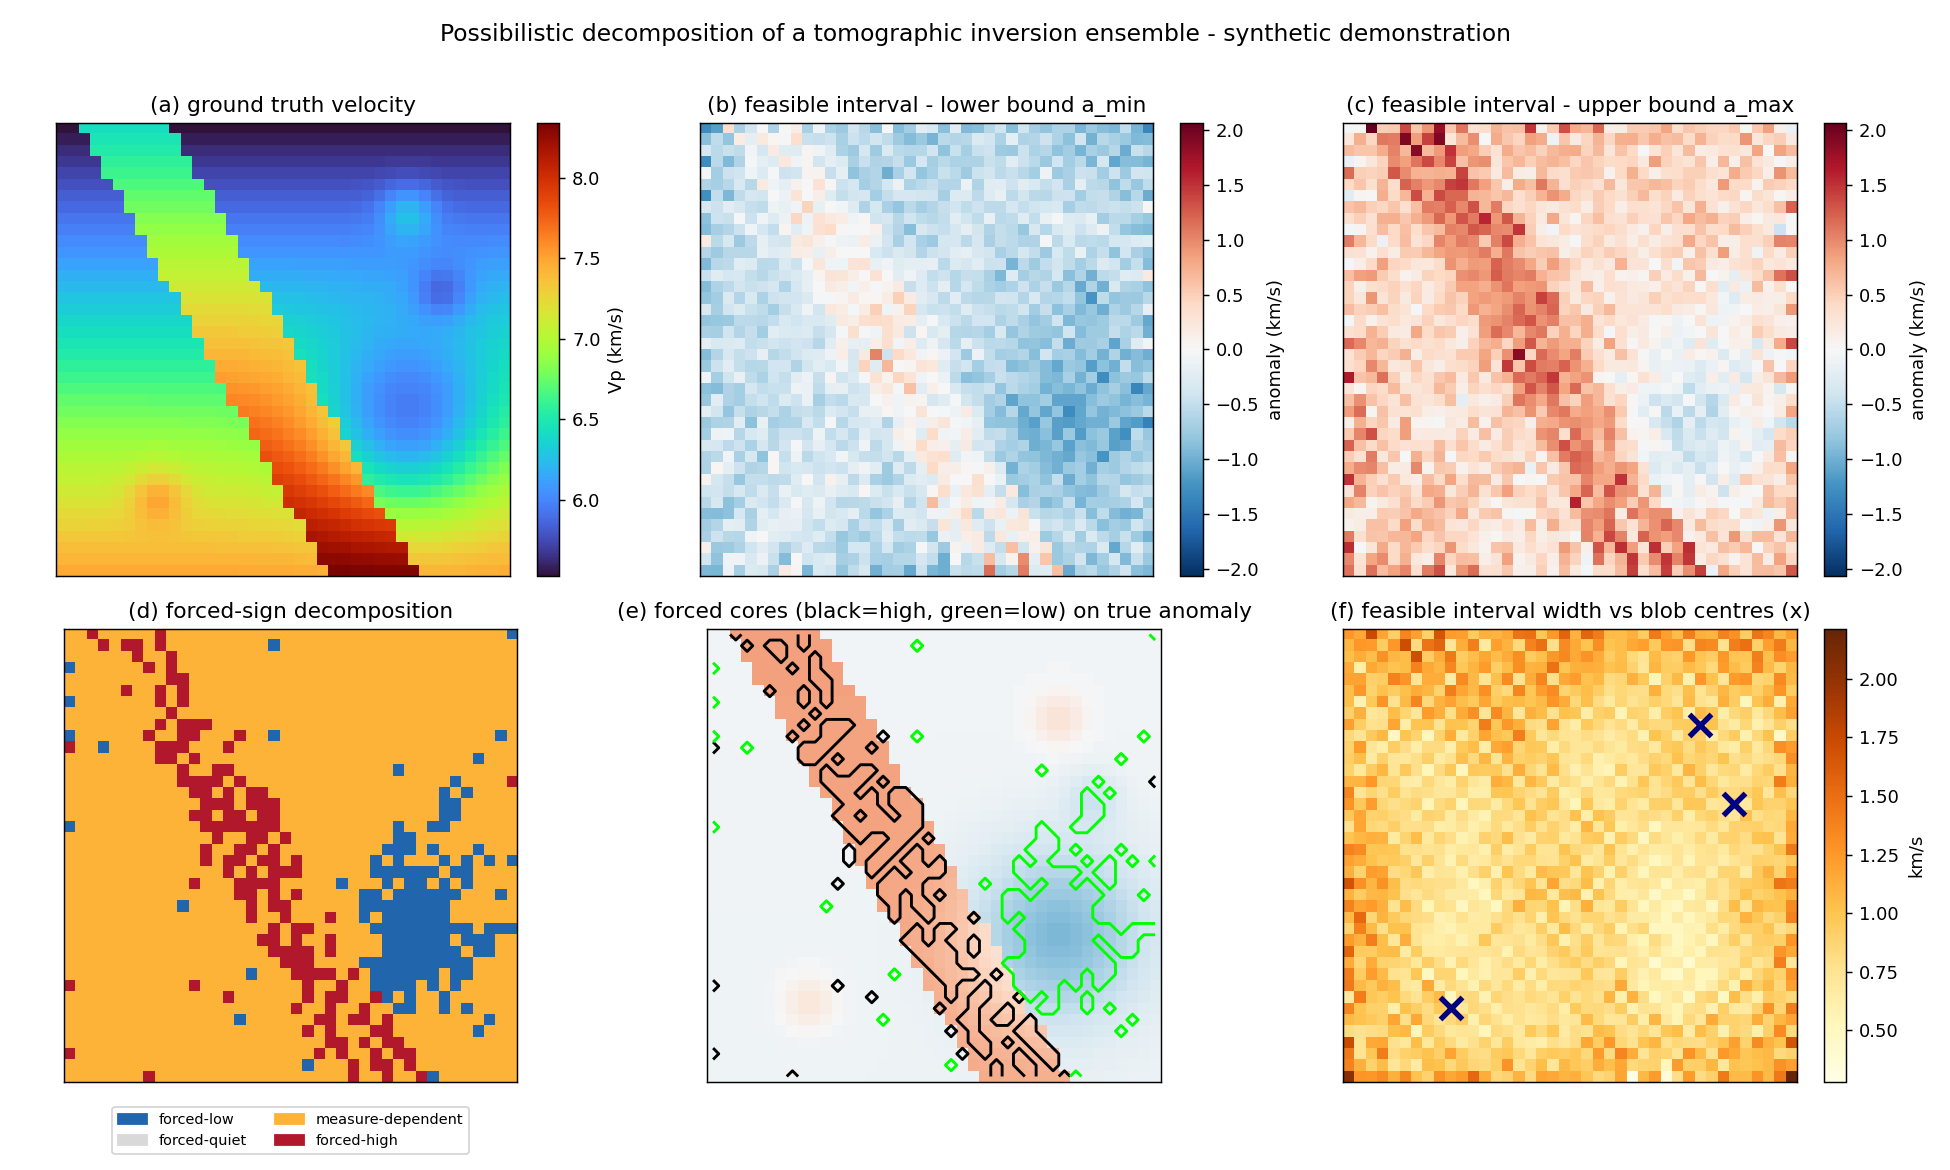
\includegraphics[width=\linewidth]{possibilistic_decomposition.png}
\caption{The straight-ray (linear) demonstration. Panel~(d) is the
decomposition; panel~(e) shows the forced cores landing on the true features.}
\label{fig:demo1}
\end{figure}

\section{Demonstration 2 --- Eikonal operator (nonlinear)}

The straight-ray operator is exact only in a homogeneous medium. The faithful
operator is the Eikonal first-arrival solver---the operator class your
\file{FMM.cpp} implements. First-arrival rays bend: toward fast structure, away
from slow (Figure~\ref{fig:rays}). \file{eikonal.py} provides it (Fast Marching
Method solver $+$ ray-path Fr\'echet kernel), standalone and self-tested.

\begin{figure}[htbp]
\centering
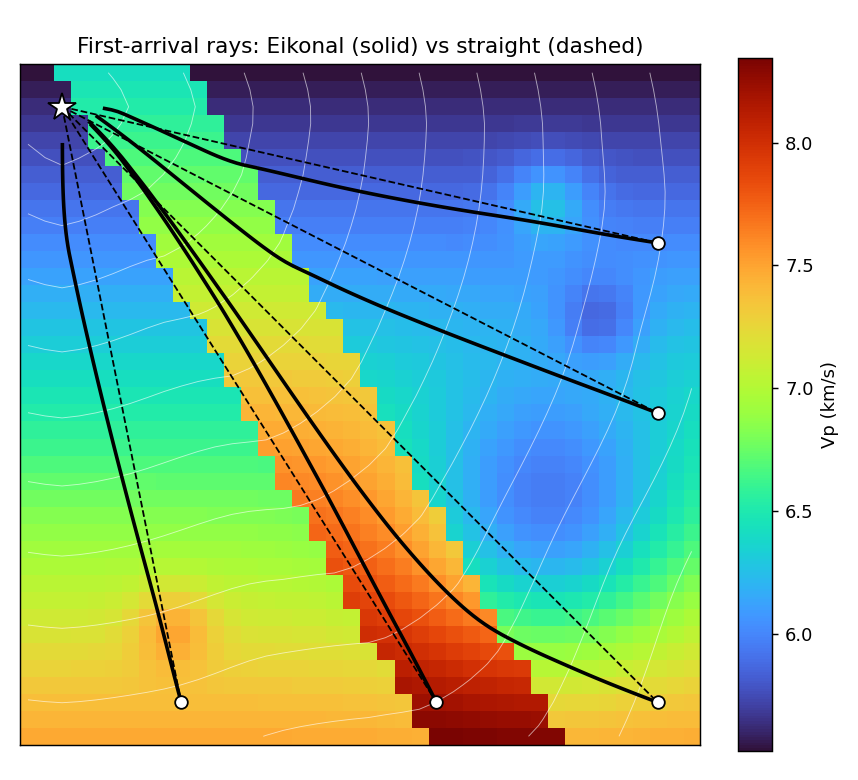
\includegraphics[width=0.62\linewidth]{fig_ray_bending.png}
\caption{Why the forward operator matters. Solid: Eikonal first-arrival rays,
bending through the medium. Dashed: the straight-ray approximation.}
\label{fig:rays}
\end{figure}

Because travel time is now a nonlinear functional of slowness, the one-shot
linear solve is replaced by an iterative Levenberg--Marquardt inversion that
recomputes the ray paths through the current model---the DGN $+$ FMM structure
of your own pipeline. Figure~\ref{fig:demo2} is the result, and the
decomposition code is \emph{identical} to Demonstration~1:

\begin{itemize}
\item \textbf{Forced cores $\sim$89\% sign-correct within the resolution
  length}, but $\sim$71--81\% strict (cell-exact). The gap is resolution-length
  blur---a forced cell one or two cells off a true feature edge, not a sign
  mistake---but the strict figure is the honest co-headline; the
  within-resolution number alone overstates the precision.
\item \textbf{The measure-dependent shell captures $\sim$76\% of the blobs.}
\end{itemize}

These figures are from the feasible-set sampler at its default operating point,
and at that operating point the forced set itself over-claims: an adversarial
stress test (\S7, point~6; \file{witness\_pass.md}, RWC-2) finds $\sim$41\% of
forced cells admit a feasible, equally-smooth, opposite-sign model. The
decomposition layer is sound and forward-model-agnostic; what is
coverage-limited is the feasible-set \emph{sampling} that feeds it (\S8).

The decomposition transferred across two genuinely different forward operators
without change. That is the load-bearing result of this note: the possibilistic
reading is a property of \emph{inversions}, not of a particular operator.

\begin{figure}[htbp]
\centering
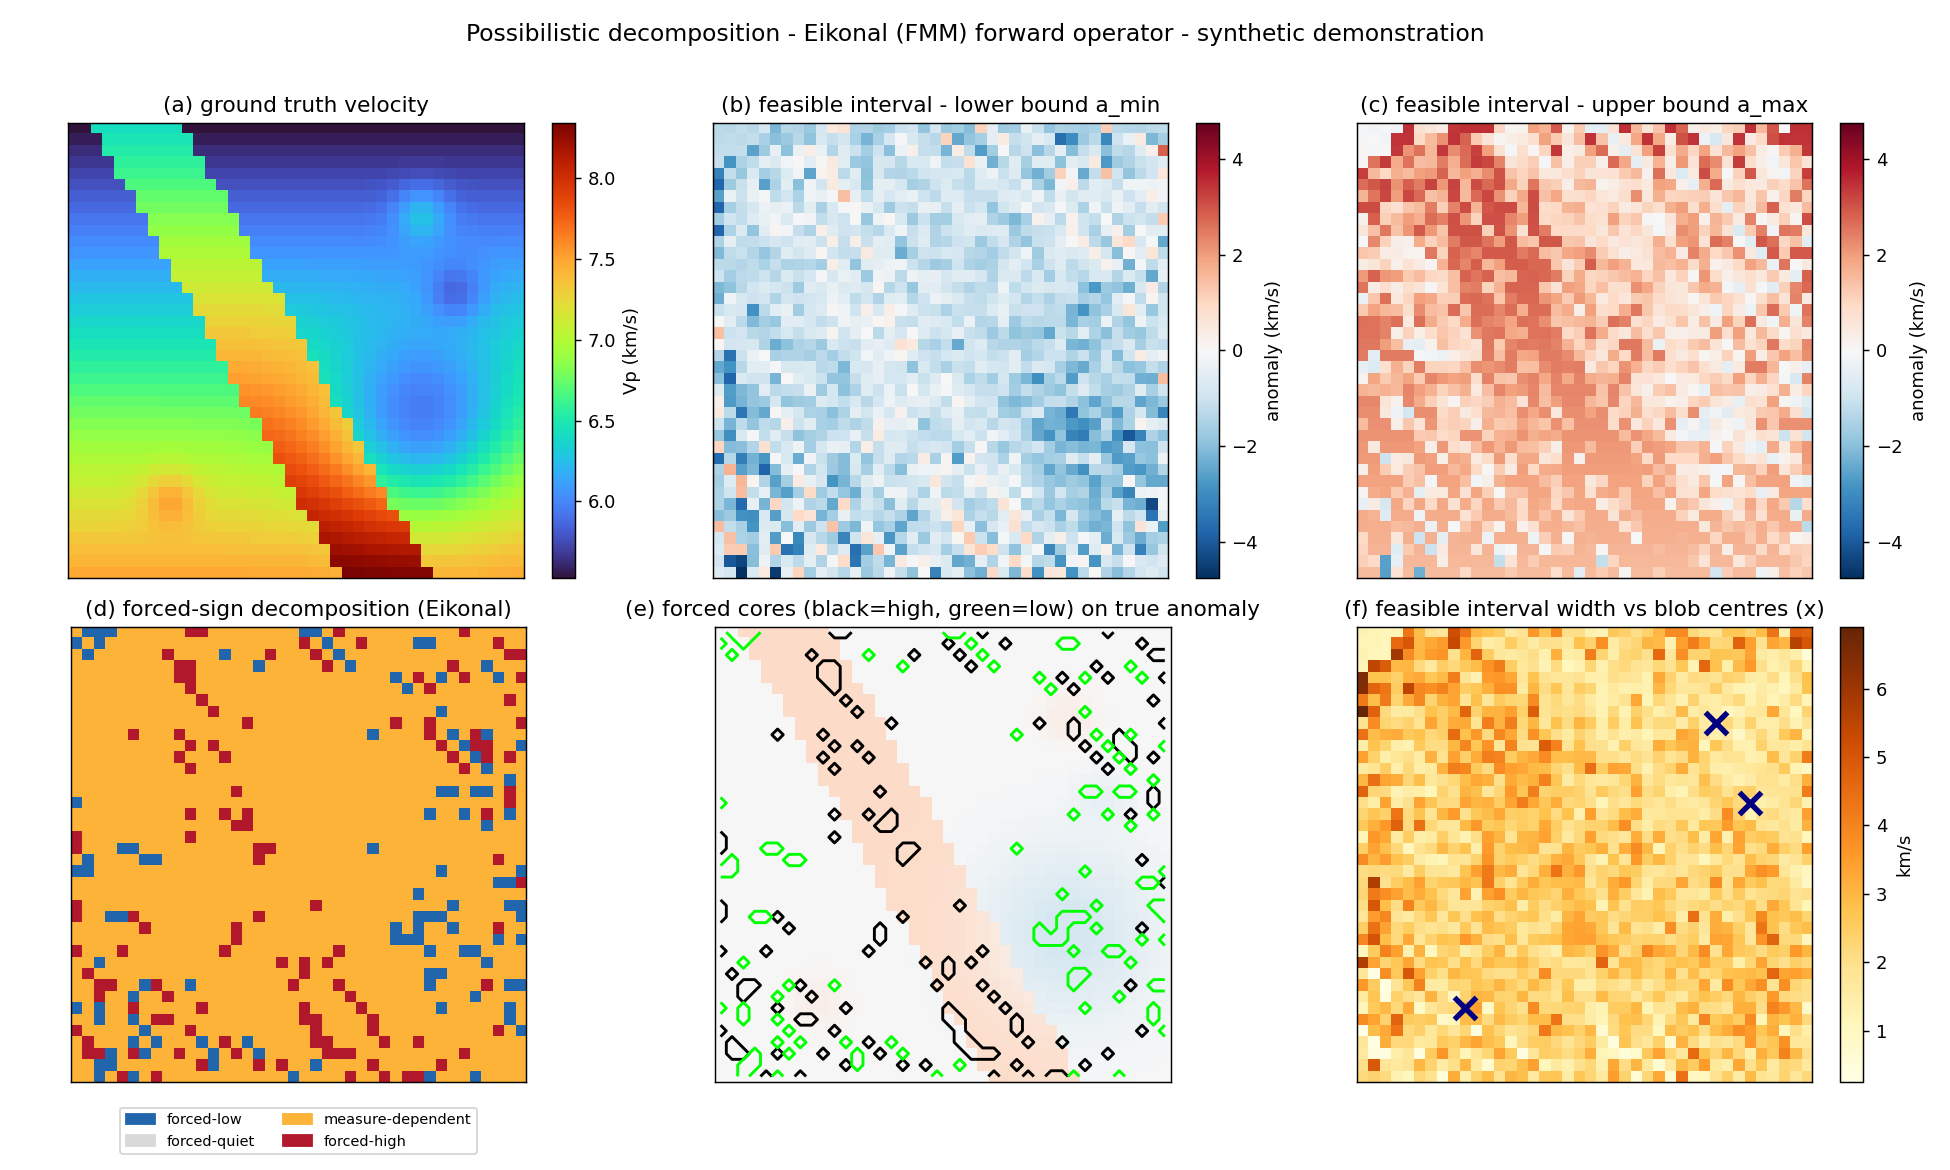
\includegraphics[width=\linewidth]{possibilistic_decomposition_eikonal.png}
\caption{The Eikonal (nonlinear) demonstration---same decomposition, faithful
operator.}
\label{fig:demo2}
\end{figure}

\section{Demonstration 3 --- real-data on the Volve walkaway VSP}
\label{sec:realdata}

Demonstrations 1 and 2 validate the methodology against synthetic ground
truth. This section asks the next question: does any of it survive contact
with a real field dataset? The \textbf{Equinor Volve open release} (North
Sea, 2018), made available under Equinor's \emph{HRS Terms and conditions
for licence to data --- Volve} (\S6.6), includes walkaway-VSP surveys for
two wells with full wireline-log suites --- independent sonic ground truth
at known locations. The data pipeline from raw SEG-Y to forced/measure-
dependent classification is shipped in the \file{volve/} subpackage of the
methodology repository; the report below is what came out of it.

\subsection{1D \texorpdfstring{$V_p(z)$}{Vp(z)} on well 15/9-F-15A --- the methodology calibrates}

Picks: STA(10\,ms)/LTA(100\,ms) trigger with AIC refinement on the
Z-component geophone traces, 1215 ok of 1248 (97.4\,\% yield; the 33
no-trigger traces are the 5 far-offset sources). Ensemble: 30 random-reference
Eikonal Gauss--Newton members on 45 depth bins (70\,m), envelope $[1.5,
5.5]$\,km/s, smoothness correlation 250\,m. Validation: the LAS bundle's
\file{DT-EDIT} sonic curve, checkshot-stretched to TVD.

Headline numbers, real data:

\begin{itemize}
\item \textbf{Per-bin ensemble $V_p$ interval covers the wireline sonic in
  36/45 bins (80.0\,\%).}
\item \textbf{Held-out arrival calibration: 228/243 (93.8\,\%) of held-out
  pick times fall inside the ensemble's predicted-time interval.}
\item Signed error (ensemble median minus sonic) median $+0.29$\,km/s; the
  ensemble runs slightly slow at depth, consistent with the first-order FMM
  solver and the 1D-along-bore parameterization.
\end{itemize}

\begin{figure}[htbp]
\centering
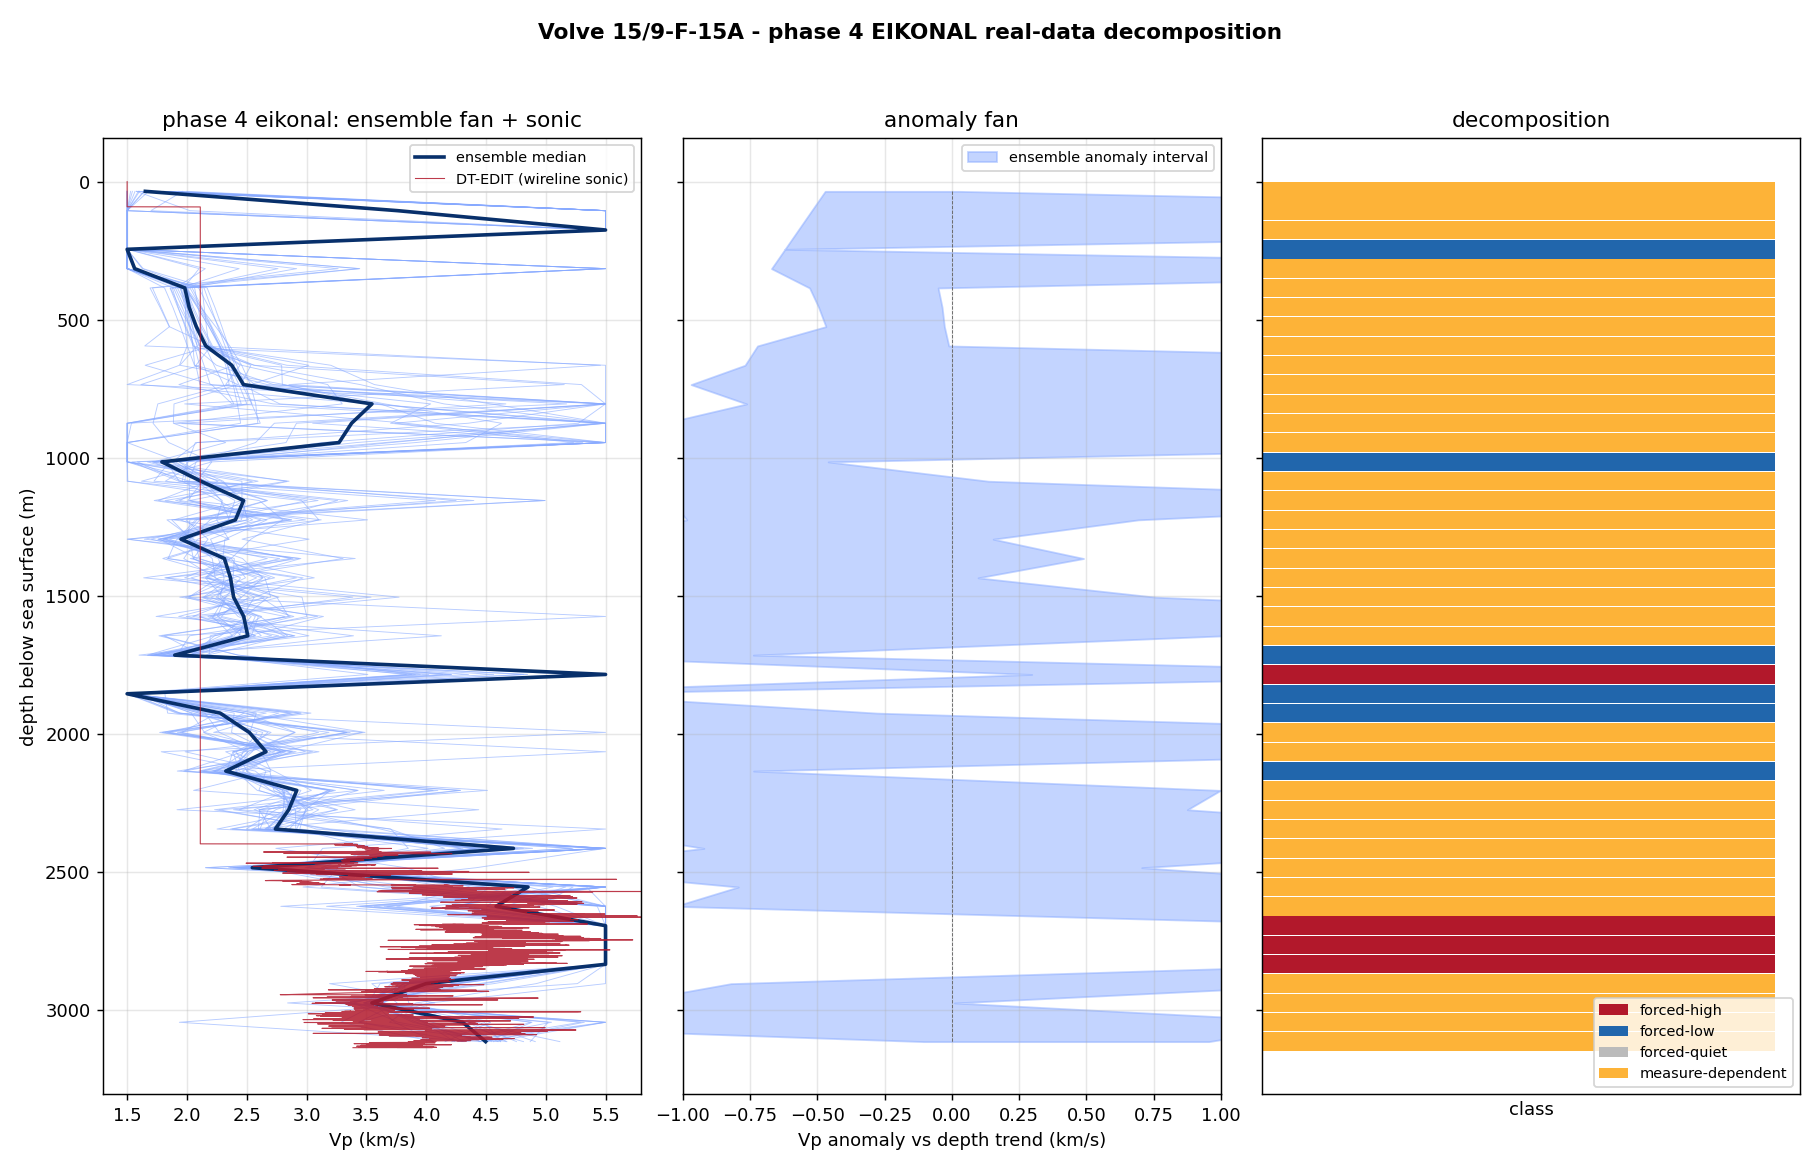
\includegraphics[width=\linewidth]{volve_phase4_decomposition.png}
\caption{Possibilistic decomposition on the 15/9-F-15A walkaway VSP. Left:
30-member ensemble $V_p(z)$ fan against the DT-EDIT wireline sonic. Centre:
the per-bin anomaly interval relative to the depth trend. Right: the
forced-high / forced-low / measure-dependent classification. The ensemble's
per-bin $V_p$ interval covers the wireline sonic in $80\,\%$ of depth bins,
and the held-out arrival calibration lands at $93.8\,\%$ --- at the rate
the possibilistic frame claims for full-coverage forecasts.}
\label{fig:phase4_decomp}
\end{figure}

That is the ``methodology mechanically works on real first arrivals''
outcome. Calibration matches the methodology's claim; the operator-relative
caveats of \S9 apply unchanged.

\subsection{2D joint inversion on F-15A + F-11 T2 --- structural misspecification surfaces}

Two wells are 1061\,m apart laterally; combined they sample depths
$\approx$\,130--4530\,m. Promoting to 2D $V_p(w, z)$ on a (well-line,
depth) grid through both wellheads multiplies the model space $\sim$180$\times$
(45 bins $\rightarrow$ 8004 cells) without 180$\times$ more data, and
changes the inversion's character.

Three rounds of work were needed to get an honest read:

\begin{enumerate}
\item \textbf{First-cut report.} A 12-member ensemble $\times$ 2
  Gauss--Newton iterations produced sonic-inside coverage of 10\,\% at each
  well's wellhead column, a joint held-out inside rate of 23\,\%, and 79\,\%
  ``forced-quiet'' cells. The narrative on first read was \emph{``prior
  dominance in unilluminated cells.''}
\item \textbf{Triad witness pass.} A scoped brief went to three independent
  AI witnesses (Venice / Grok / ChatGPT). They converged on four interpretation
  artifacts the first read was leaning on: the anomaly baseline was the
  ensemble mean (gauge-sensitive), the sonic was sampled at the wellhead
  column instead of along the deviated bore (category error), the ensemble
  size was small (under-exploration risk), and the prior strength was not
  directly tested. ChatGPT specifically named the structural-misspecification
  hypothesis --- \emph{2D $V_p(w, z)$ on a 3D Earth} --- as the leading
  alternative.
\item \textbf{Phase A diagnostics + Phase B re-run.} Each artifact was
  tested in sequence. Switching to a wireline-derived anomaly baseline
  collapsed the 79\,\% forced-quiet to 22\,\% (the original number was
  gauge-sensitive). Sampling the sonic along the bore trajectory raised the
  F-15A sonic-inside from 10\,\% $\rightarrow$ 32\,\% (post-processing)
  $\rightarrow$ \textbf{57\,\%} (Phase B re-inversion, 30 members $\times$
  3 GN iters, looser prior). Loosening the smoothness correlation
  350 $\rightarrow$ 700\,m and the envelope 1.5--5.5 $\rightarrow$
  1.3--6.0\,km/s did \textbf{not} widen the predicted-time interval
  (21\,ms $\rightarrow$ 24\,ms) and did \textbf{not} shrink the held-out
  residual (137\,ms $\rightarrow$ 134\,ms RMS). Across all 30 members,
  \textbf{44\,\% of cells classify as forced-low against the wireline-sonic
  baseline} --- the ensemble systematically sits below the sonic, and the
  diagnosis is stable.
\end{enumerate}

\begin{figure}[htbp]
\centering
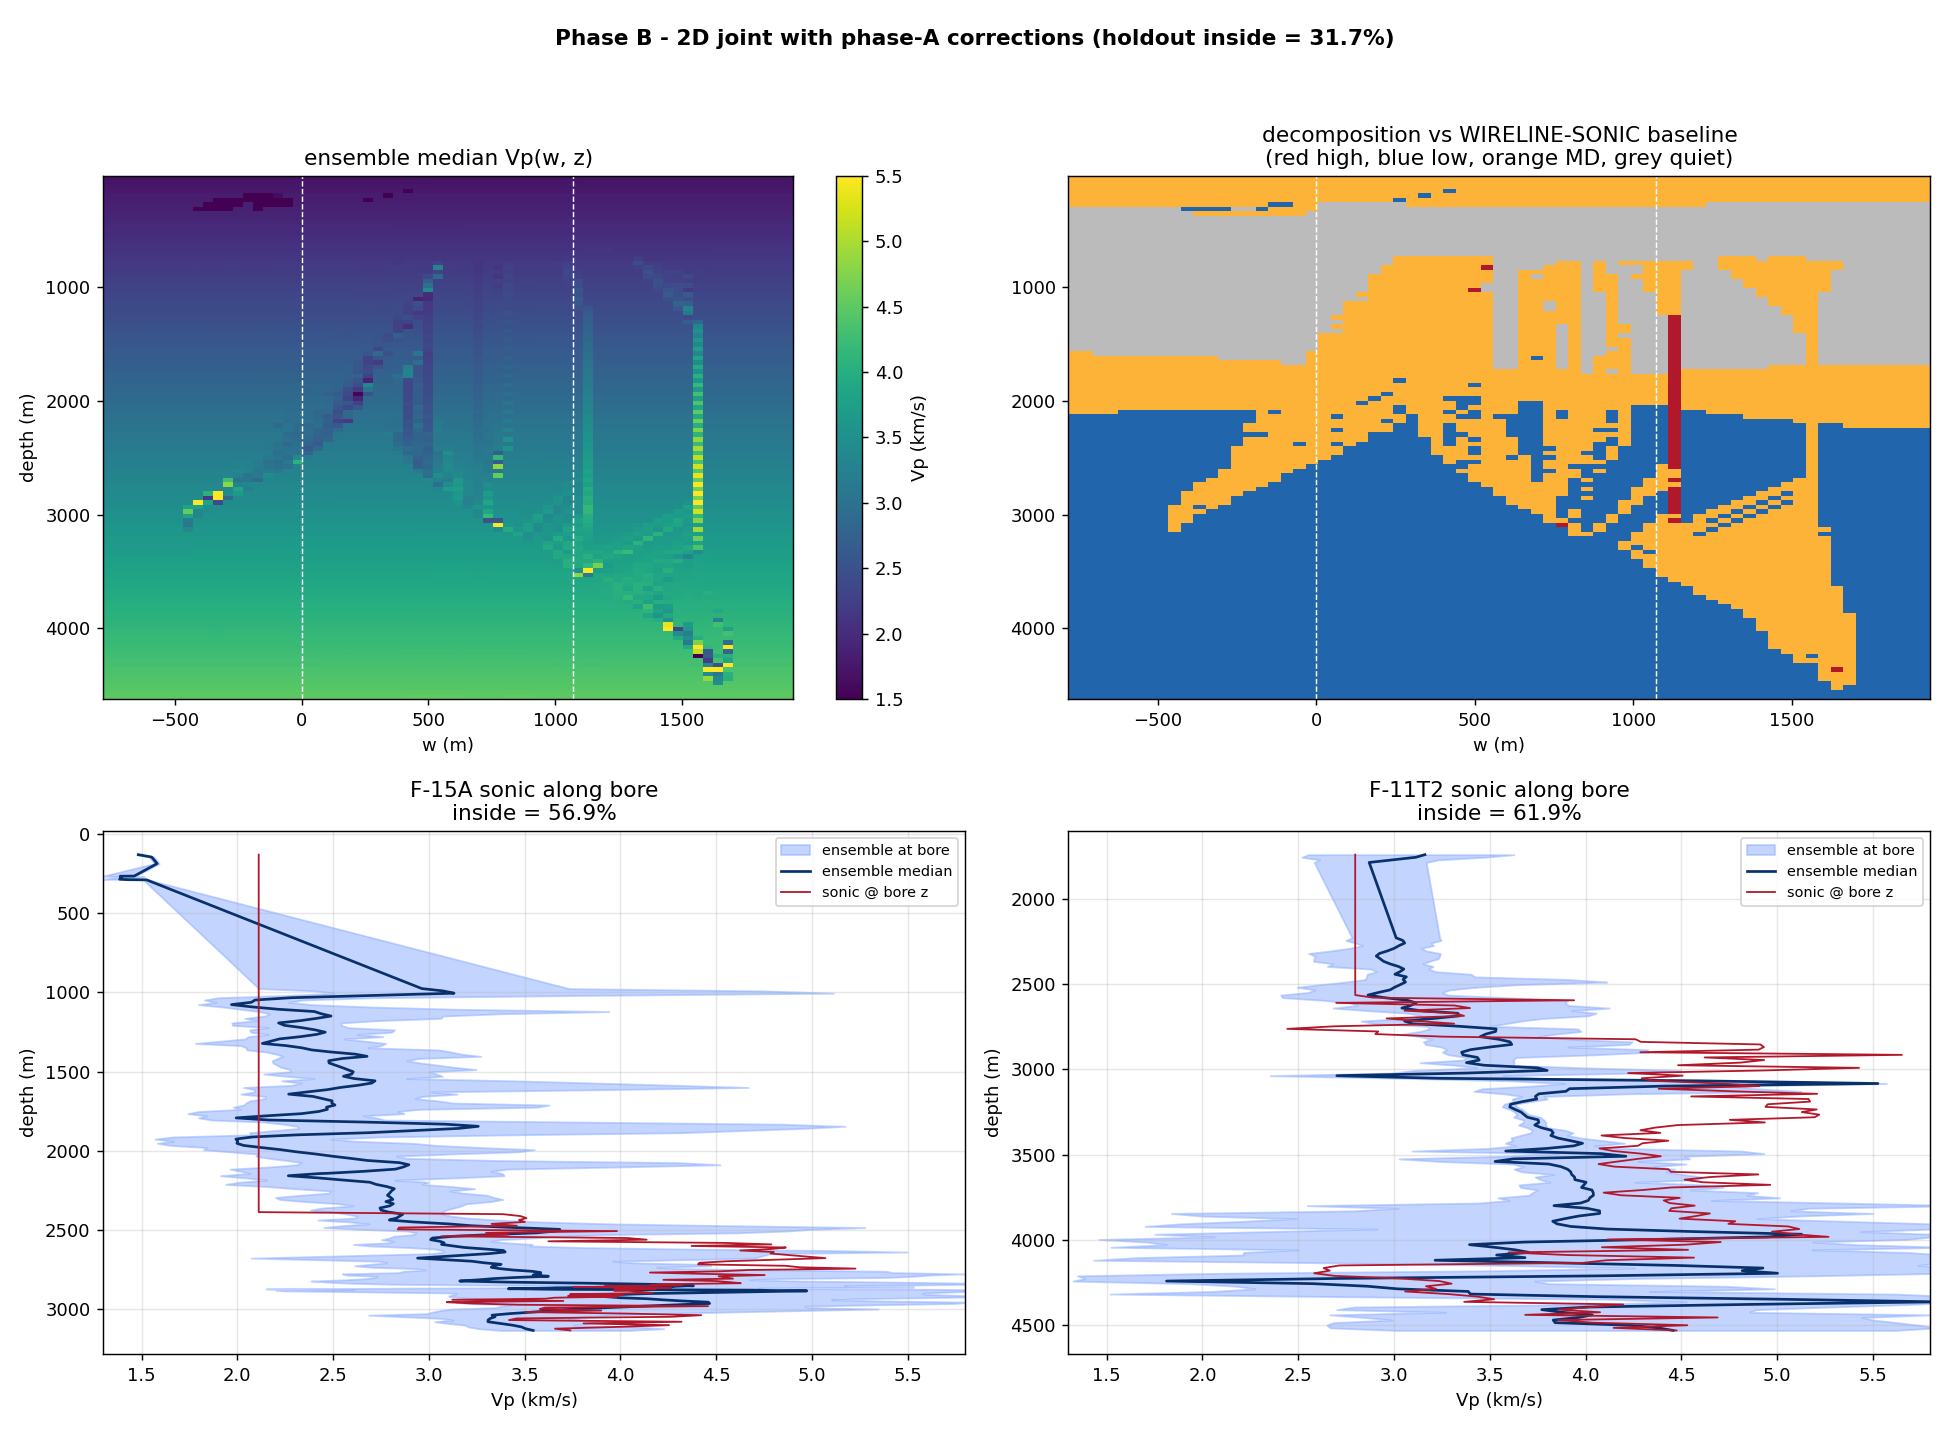
\includegraphics[width=\linewidth]{volve_phaseB_decomposition.png}
\caption{2D $V_p(w, z)$ joint inversion of the F-15A + F-11 T2 picks
(Phase B, with the witness-pass artifact corrections applied). Top:
ensemble median $V_p(w, z)$ and the forced/measure-dependent
classification versus the wireline-sonic baseline (red high, blue low,
orange measure-dependent, grey forced-quiet). Bottom: sonic-along-bore
vs ensemble at each well --- 57\,\% (F-15A) and 62\,\% (F-11 T2) inside
the ensemble interval. The persistent 44\,\% forced-low (blue) at depth
is the diagnostic: 2D $V_p(w, z)$ is structurally insufficient for the
3D Earth at this geometry, and the methodology reports it.}
\label{fig:phase5_decomp}
\end{figure}

The methodology is doing what it should. The ensemble has ten effective
dimensions (it is exploring genuine diversity, not collapsing onto a single
member), and yet every member fits the picks but sits below the sonic at
depth. The 44\,\% forced-low survives prior loosening because the binding
constraint is the parameterization itself, not the prior strength. \emph{That}
is what ``the forward operator (or parameterization) is the load-bearing
approximation'' looks like in real data, and the decomposition correctly
flags it.

\subsection{The witness pass as part of the method}

The witness pass and the four corrections it produced are themselves part of
the methodology contribution. The discipline is: \emph{publish the
first-cut interpretation, run external witnesses on the brief, run the
diagnostics they recommend, retract the parts that were gauge-sensitive or
confounded, re-run with the corrections, and re-report.} This was the
second time in the methodology's development that triad witnesses caught an
interpretation drift (the first was the possibilism note's figure pass with
Crane and Martin); the practice is now treated as a step in the workflow,
not an extra.

\subsection{Head-to-head: possibilistic vs Bayesian vs neural-net}

On the F-15A 1D problem, under matched physics (Eikonal FMM forward),
matched prior (smooth random $V_p(z)$ on 45 bins, envelope 1.5--5.5\,km/s,
smoothness correlation 250\,m), and matched data (the same 1215 picks),
three different representations of inversion uncertainty:

\begin{center}
\begin{tabular}{lrr}
\hline
Method                                       & Sonic-inside & Holdout median RMS \\
\hline
posdec (feasibility interval, 30-member)     & \textbf{80.0\,\%} &  179\,ms \\
MCMC (emcee linearized, 90\,\% credible)     &  55.6\,\% &  179\,ms \\
MCMC (95\,\% credible)                       &  64.4\,\% &  (same) \\
NN (MLP, MC dropout, 90\,\% band)            &   6.7\,\% &  490\,ms \\
NN (MC dropout, 95\,\% band)                 &   8.9\,\% &  (same) \\
\hline
\end{tabular}
\end{center}

\begin{figure}[htbp]
\centering
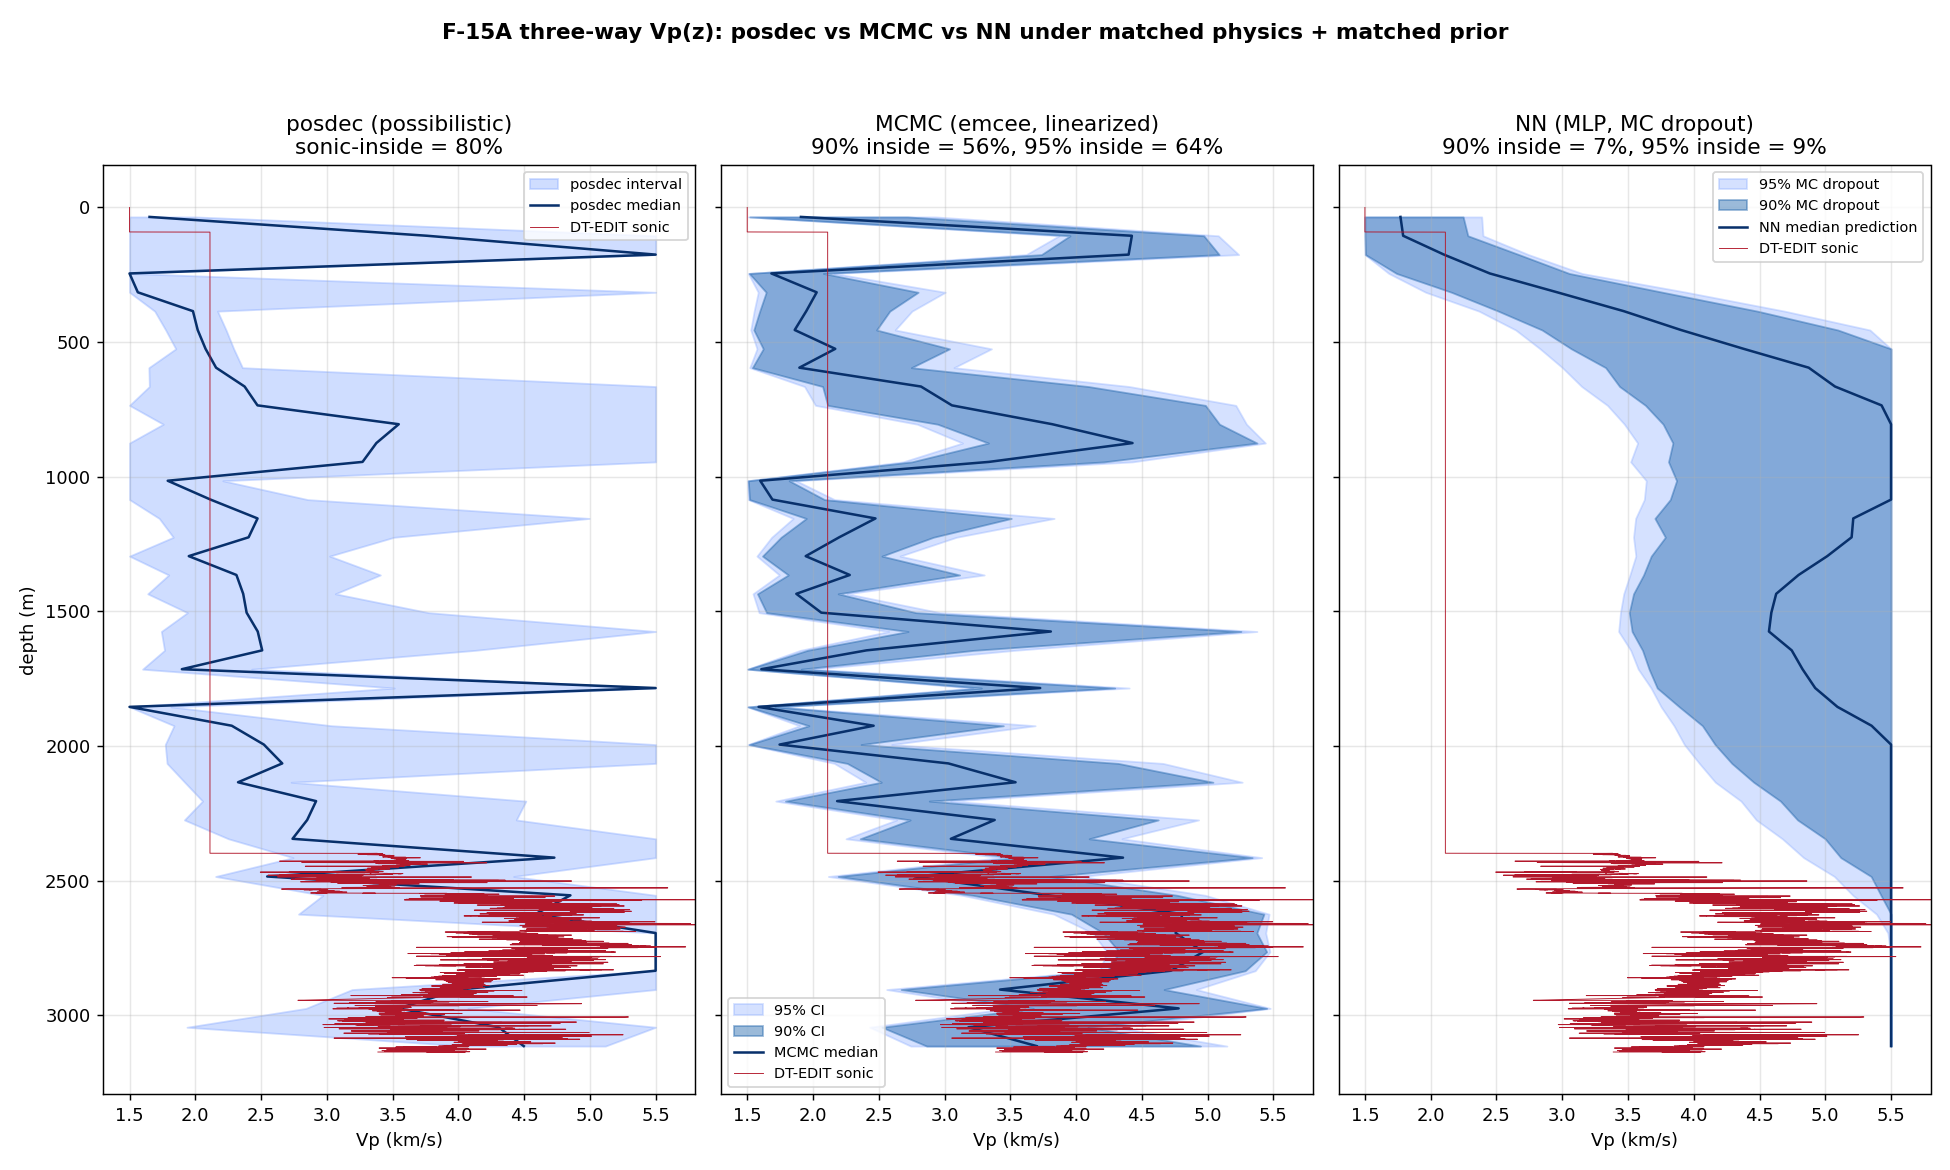
\includegraphics[width=\linewidth]{volve_threeway.png}
\caption{Three uncertainty representations on the same inverse problem.
posdec feasibility interval is widest and covers the sonic at the rate the
possibilistic frame claims (80\,\%). MCMC's Bayesian credible intervals
contract more tightly because the Gaussian likelihood imposes shape
constraints beyond mere feasibility; same central estimate (179\,ms
holdout RMS) but more confident uncertainty. MC dropout on a supervised
MLP trained on matched-prior synthetic data captures epistemic uncertainty
within the training distribution and is blind to real-data distributional
shift: the dropout band is narrow and the median prediction is also off
the real trend (490\,ms holdout RMS).}
\label{fig:threeway}
\end{figure}

The point is not ``which method is best.'' It is that \textbf{each choice
of uncertainty representation gives a quantifiably different account} of
the same inverse problem --- same physics, same prior, same data --- and
the choice is methodologically load-bearing. Brian's ORSI Tier-1
sensitivity work on the synthetic side flagged the analogous
load-bearing-ness of the smoothness prior (\S7 item 7,
Figure~\ref{fig:sensitivity}); the three-way head-to-head is its real-data
analog. Possibilistic is the most conservative; that is the methodology's
design, and on this real-data test it delivers the calibration its frame
claims.

\subsection{Honest scope of the real-data section}

\begin{itemize}
\item One field (Volve), two wells. The 1D F-15A result calibrates; the
  2D joint result correctly diagnoses parameterization limits.
\item Eikonal first-order FMM, not finite-frequency or full-waveform.
\item The MCMC comparator uses a linearized forward (matrix--vector per
  step) at the ensemble-median reference, not a full nonlinear chain;
  emcee is run with 100 walkers $\times$ 3500 steps.
\item The NN comparator is a stock MLP trained on synthetic
  eikonal-forward picks from the matched prior, MC dropout for uncertainty.
  NN tomography state-of-the-art (normalizing-flow posteriors, Bayesian
  NNs, PINNs) was not invoked; that is a separate scope.
\item A structurally different parameterization (full 3D, anisotropy,
  finite-frequency) was not tested. Brian's ORSI evaluation explicitly
  recommends that as the natural extension, paired with a domain
  collaborator.
\end{itemize}

\subsection{Data attribution and licence}
\label{sec:realdata-licence}

The data used in this section is the \textbf{Equinor Volve open dataset} ---
the walkaway-VSP bundles for wells \textbf{15/9-F-15 A} and
\textbf{15/9-F-11 T2} under \file{08.VSP\_VELOCITY}, and the corresponding
petrophysical-interpretation bundles under
\file{05.PETROPHYSICAL INTERPRETATION}. The data is licensed by
\textbf{Equinor ASA}, \textbf{ExxonMobil Exploration \& Production Norway AS},
and \textbf{Bayerngas Norge AS} (the ``former Volve license partners'')
under the \emph{HRS Terms and conditions for licence to data --- Volve}
(the ``HRS T\&C''). The HRS T\&C is a CC BY 4.0--derived licence with two
material modifications: (a) the Licensed Material may not be sold, and
(b) the licence covers all data in the dataset whether or not it is by law
covered by copyright.

The work in this section falls within the permitted scope of \S3 of the
HRS T\&C:
\begin{itemize}
\item The Licensed Material is used to \textbf{produce Adapted Material}
  (first-arrival picks, eikonal feasibility ensembles, possibilistic
  forced/measure-dependent classifications, MCMC and NN comparators, and
  the figures herein), which the HRS T\&C explicitly permits (\S3.1).
\item The Adapted Material and the original Licensed Material can be
  \textbf{shared openly} under the HRS T\&C's Sharing clause (\S3.3). The
  methodology repository's own licence (where applicable to derived data)
  does not prevent recipients from complying with the HRS T\&C.
\item The presentation here is \textbf{not misleading or distorted}
  (\S3.2): every per-well, per-method calibration number, residual, and
  forced-set fraction is reported as measured, with its scope caveats
  inline.
\end{itemize}

Nothing in this section (or elsewhere in this note) \textbf{constitutes or
implies endorsement} of this work by Equinor or the former Volve licence
partners (HRS T\&C \S4). The licence partners are credited solely as the
data providers; the methodology, the inversion results, and the
interpretive narrative are the author's, with the honest-scope caveats of
the previous subsection and of \S9 applying.

\textbf{Citation and link.} The official HRS Terms and conditions document
is available from Equinor's open-data portal at
\url{https://www.equinor.com/energy/data-sharing}. The dataset itself
(``the Volve Data Village'') is described in Exhibit~1 of the HRS T\&C;
the specific bundles used here are folders 8 and 9 of that exhibit
(\file{Well\_logs} and \file{Well\_logs\_pr\_WELL}). When citing this
work, please also cite Equinor's release per the HRS T\&C attribution
requirement.

\section{What building it surfaced --- the discipline the method needs}

A method that always says ``yes'' is a gimmick. This one has real failure
modes, and finding them is how I know it has content. Each was surfaced by a
synthetic run failing honestly; each is now documented in the script headers.

\begin{enumerate}
\item \textbf{The ensemble must sample the feasible set's diversity, or it
  certifies its own bias.} An ensemble built by varying damping \emph{strength}
  alone shares a bias in the data-null directions; the intersection then stamps
  that shared bias ``forced.'' The fix is many random references.
\item \textbf{Sample where the data is actually fit}---at the
  misfit $=$ noise level. An over-damped ensemble has had data-resolved
  structure regularized away.
\item \textbf{``Forced'' is a sign statement off the interval, not a hard
  threshold.} A single anomaly-magnitude cutoff is brittle; the feasible
  interval is the honest object.
\item \textbf{Precision is honest only at the resolution length.} Every
  feasible model inherits the same forward-operator blur; the forced core is
  correct to within roughly one cell, not cell-exact.
\item \textbf{Feasible models must be physically plausible --- smooth.} The raw
  null space of a ray (line-integral) operator is dominated by high-frequency
  checkerboard modes the operator cannot see. Those fit the data but are not
  admissible Earth models; perturbing freely in them injects unphysical
  speckle. A feasible model is data-fitting \emph{and} smooth.
\item \textbf{The forced set is coverage-gated --- and the gate is
  measurable.} A forced label asserts that \emph{every} feasible model agrees;
  an ensemble that under-samples the feasible set will agree spuriously and
  over-claim. Two checks quantify this (\file{witness\_pass.md}, RWC-1 and
  RWC-2): the forced set converges only above an ensemble-coverage
  threshold---here $N \approx 250$ sampled models for a $40\times40$ grid---and
  at the default operating point an adversarial stress test finds $\sim$41\% of
  forced cells \emph{false-forced} (a feasible, equally-smooth, opposite-sign
  model exists). A forced claim is honest only with its coverage-adequacy curve
  attached.
\item \textbf{The Tier-1 admissibility bounds are themselves load-bearing
  --- and the dependence is now measured.} The possibilistic layer is defined
  relative to a hard admissibility envelope
  (\file{geophysical\_invariants.md}): a velocity range, a positivity
  condition, a smoothness preference enforced by the sampler. The split is
  only as data-forced as those bounds are data-independent. The natural worry
  that the smoothness preference sneaks regularization into the possibilistic
  layer is now answered quantitatively
  (\file{sensitivity\_tier1.py}, Figure~\ref{fig:sensitivity}). Tightening
  the velocity floor $V_{P,\min}$ from $2.0$ to $3.0$ km/s drops the
  forced-high Jaccard to $0.27$; the $V_{P,\max} = 9$ km/s ceiling is
  saturated (every member touches it); and the smoothness preference is
  load-bearing --- at the $25\%$ smoothness percentile the smoothness-kept
  ensemble gives $J(\textrm{forced-high}) = 0.36$ versus $J = 0.77$ for a
  random-size-matched control, a $\sim$0.4 Jaccard gap that is
  \emph{specifically} the smoothness preference rather than the generic
  smaller-sample narrowing. The Tier-1 envelope is therefore reported
  alongside the coverage-adequacy curve, not assumed.
\end{enumerate}

\begin{figure}[h]
\centering
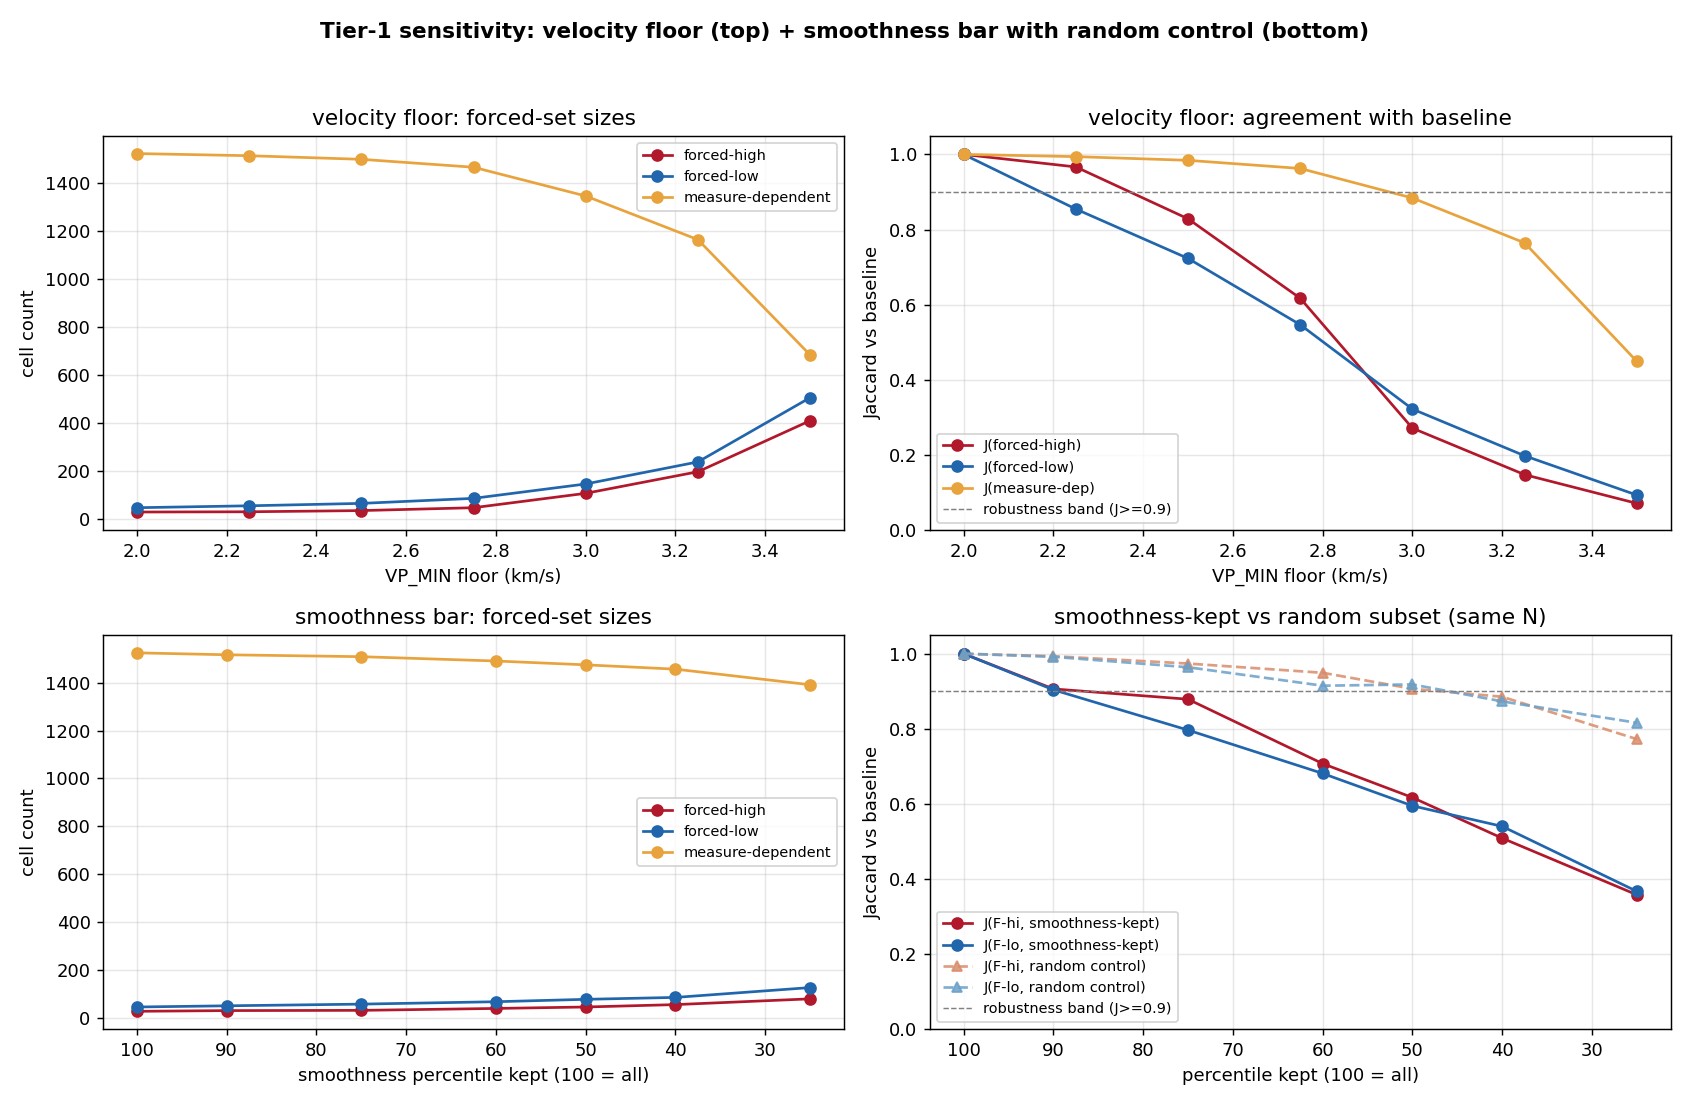
\includegraphics[width=0.95\linewidth]{sensitivity_tier1.png}
\caption{Tier-1 sensitivity sweep on the 396-member RWC-1 ensemble. Top
row: velocity-floor sweep (the $V_{P,\max}$ ceiling is saturated at
$100\%$ and not separately sweepable). Bottom row: smoothness-percentile
sweep with a random-subset control of the same $N$. The smoothness-kept
Jaccard sits below the random-control curve at every $p$, identifying the
smoothness preference as a load-bearing admissibility choice --- not
merely a sampler convenience.}
\label{fig:sensitivity}
\end{figure}

These are not patches. They are the methodology's anti-anchoring
discipline---the same one that, in the Closure programme, keeps a derivation
from quietly tuning itself to the answer it wants.

\section{The open frontier --- and where you come in}

Here is the honest seam, and it is the reason this is a note to \emph{you} and
not a finished claim.

The linear straight-ray case has a clean, exact answer: the operator is fixed,
$G^{\top}G$ eigendecomposes once, and the feasible set is parametrized directly.
The nonlinear case does not. Sampling the feasible set of a nonlinear inverse
problem---getting genuine diversity in the data-null directions without
injecting artifacts---is itself a hard problem. Building Demonstration~2 walked
straight into it: a naive Levenberg--Marquardt ensemble shares an
inversion-dynamics bias; fixing that needs explicit, physically-constrained
feasible-set sampling. I have a working version, but I would not call the
nonlinear feasible-set sampler solved.

This is exactly the territory of transdimensional / reversible-jump MCMC
tomography (Bodin \& Sambridge, 2009 onward)---methods built precisely to
produce a genuine posterior ensemble. And it is where ZTM already lives: your
\file{runs=20} top-level Monte Carlo \emph{is} a feasible-set sampler. A
coverage study on the synthetic problem (\file{witness\_pass.md}, RWC-1) now
puts a number on the question: the forced set stabilizes only near
$N \approx 250$ sampled models, and a 20-run ensemble sits at roughly three
times the converged forced-set size---20 runs is far short of coverage
adequacy. So the open question is no longer \emph{whether} the sampler needs
upgrading but \emph{to what}: whether a transdimensional sampler reaches the
coverage the forced/measure-dependent split requires, on real data, at
tractable cost.

That question is not mine to answer from the outside. It needs your inversion
expertise, your code, and your data. My contribution is the possibilistic
reading and the formal scaffolding behind it; yours is the geophysics and the
instrument. Neither half is sufficient alone. That is the collaboration I am
proposing---not ``adopt this method,'' but ``here is a method, validated in the
linear case, and here is the concrete nonlinear problem your own pipeline is
already engaging. Let us solve that part together.''

\section{Honest scope}

\begin{itemize}
\item Everything here is \textbf{synthetic}. The demonstrations validate the
  \emph{method} against known ground truth; they are not a result about the
  real Earth.
\item The Eikonal solver is \textbf{first-order FMM}. Its $\sim$2\% mean
  accuracy is fine for a forward-model-agnostic demonstration; your FMM-VFD
  hybrid is the production-grade version.
\item Two dimensions, modest velocity contrasts, a single noise realization.
  None of the conclusions depend on scale, but none have been \emph{tested} at
  scale.
\item The forced/measure-dependent split is \textbf{operator-relative}: it
  reports what is forced \emph{given a forward operator}. An operator with
  systematic error propagates that error into the forced set. This is not a
  defect of the method---it is the method correctly reflecting the
  operator---but it means the operator's fidelity is load-bearing.
\item The \textbf{forced set is coverage-gated}. It is trustworthy only above
  an ensemble-coverage threshold (RWC-1: $N \approx 250$ here); below it the
  sampler over-claims (RWC-2: $\sim$41\% of forced cells false-forced at the
  default operating point). The demonstrations are reported at that default
  point and so over-state the forced set. The decomposition layer is
  sound---what is coverage-limited is the feasible-set \emph{sampling} that
  feeds it; a forced claim must travel with its coverage-adequacy curve.
\item The forced/measure-dependent split is \textbf{conditional on the
  Tier-1 admissibility bounds}. Both the velocity envelope (the
  $V_{P,\max} = 9$ km/s ceiling is saturated and the floor is binding well
  above the methodology's generous default) and the sampler's smoothness
  preference shift the decomposition quantifiably (\S7 item 7,
  Figure~\ref{fig:sensitivity}, \file{sensitivity\_tier1.py}). A
  published forced/measure-dependent map travels with its Tier-1 envelope
  \emph{and} its coverage-adequacy curve; either, varied within a
  plausible range, changes the result.
\end{itemize}

\section*{Acknowledgements}

The Tier-1 sensitivity finding (\S7 item 7, Figure~\ref{fig:sensitivity})
is owed to \textbf{Brian Crabtree}, whose ORSI / ORSI$\Omega$ propagation
pass on the shipped artifact named the smoothness-as-Tier-1-admissibility
concern with enough specificity to be answered quantitatively. The
coverage-certificate discipline (\S7 item 6), modular decomposition library
(\file{posdec}), and the linear-case exact regression are likewise direct
consequences of his propagation steps. The errors that survived are mine.

\section*{Appendix A --- The split as an instrument}

The main text draws the possibilistic / probabilistic split in model
space---$F$ as a set, a feature forced or measure-dependent according to where
$F$'s projection falls (Figures~\ref{fig:feasible}--\ref{fig:compose}). Readers
who think in terms of estimators and their inputs may find the same split
crisper drawn as an \emph{instrument}. The possibilistic report is a function
of $F$ alone. The Bayesian report is a function of $F$ \emph{and} a measure
$\mu$---a knob the data never set. Turn the knob and a measure-dependent
feature's reported sign swings across zero; a forced feature's reading does not
move, because the knob is not wired to it. Nothing here is new---it is
Figure~\ref{fig:reports} again, in a different register---but the register
makes one thing plain: the disagreement two defensible analysts can reach is
located entirely in the knob, and the knob is not data.

\renewcommand{\thefigure}{A.\arabic{figure}}
\setcounter{figure}{0}
\begin{figure}[htbp]
\centering
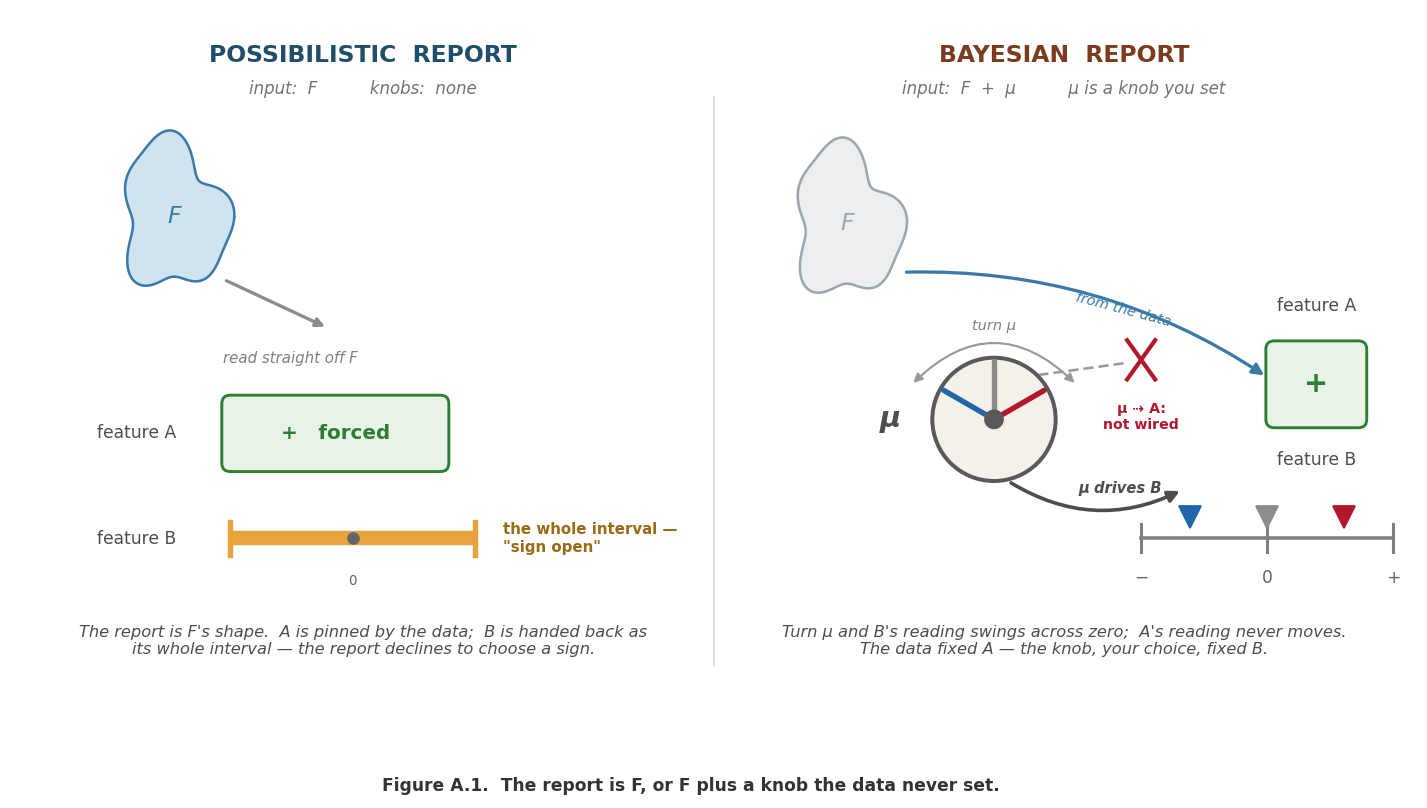
\includegraphics[width=\linewidth]{fig_two_reports_dial.png}
\caption{The possibilistic / Bayesian split as an instrument. The
possibilistic report is a function of $F$ alone---no knob. The Bayesian report
needs a measure $\mu$, a knob the data did not set: turning it swings feature
B's reported sign across zero, while feature A's reading does not move---the
knob is not wired to it.}
\label{fig:dial}
\end{figure}

\section*{Pointers}

\begin{itemize}
\item \file{geophysical\_invariants.md} --- the stratified constraint set.
\item \file{synthetic\_demo.py}, \file{synthetic\_demo\_eikonal.py} --- the two
  demonstrations.
\item \file{eikonal.py} --- the standalone Eikonal forward operator (self-test:
  \file{uv run python eikonal.py}).
\item \file{decomposition\_exact.jl} --- the decomposition layer formalized in
  exact \texttt{Rational\{BigInt\}} arithmetic (Julia); \file{classify} proven
  total, exclusive, and exhaustive, the feasible-interval properties
  exact-verified.
\item \file{c/} --- a dependency-free C port of the whole method: the forward
  operators, the Levenberg--Marquardt inversion over a hand-rolled
  dense-Cholesky module, the feasible-set sampler, and the decomposition,
  pulled together by \file{possibilistic\_inversion.c}.
\item \file{witness\_pass.md} --- the synthesis witness pass: an adversarial
  external review of the method by three independent models, and the two
  Required Witness Checks it carried, \file{rwc1\_forced\_stability.py} and
  \file{rwc2\_disconnected\_test.py}.
\item \file{inverse\_born\_methodology.md} (Closure Forces Structure
  programme) --- the source of the two-layer possibilistic / probabilistic
  discipline.
\item Bodin, T. \& Sambridge, M. (2009), \emph{Seismic tomography with the
  reversible jump algorithm}, Geophys.\ J.\ Int.\ --- the
  transdimensional-sampling reference.
\item Abatchev, Z. (2019), ZTM/TFM, UCLA --- the joint seismic$+$gravity
  inverter this note is in conversation with.
\end{itemize}

\end{document}
